\documentclass[serif, aspectratio=169]{beamer}
\usepackage[T1]{fontenc} 
\usepackage{fourier}
\usepackage{hyperref}
\usepackage{latexsym,amsmath,xcolor,multicol,booktabs,calligra}
\usepackage{booktabs} % For better table formatting
\usepackage{graphicx,pstricks,listings,stackengine}
\usepackage{listings}
\usepackage{array} 
\usepackage{colortbl}

\author{Dr.Hajialiasgari}
\title{Machine Learning}
\institute{
    Tehran University \\
    Of\\
    Medical Science
}
\date{\small \today}
\usepackage{UoWstyle}

% Define custom colors and styles for listings
\definecolor{deepblue}{rgb}{0,0,0.5}
\definecolor{deepred}{RGB}{153,0,0}
\definecolor{deepgreen}{rgb}{0,0.5,0}
\definecolor{halfgray}{gray}{0.55}

\lstset{
    basicstyle=\ttfamily\small,
    keywordstyle=\bfseries\color{deepblue},
    emphstyle=\ttfamily\color{deepred},
    stringstyle=\color{deepgreen},
    numbers=left,
    numberstyle=\small\color{halfgray},
    rulesepcolor=\color{red!20!green!20!blue!20},
    frame=shadowbox,
}

\begin{document}

\begin{frame}
    \titlepage
    \vspace*{-0.6cm}
    \begin{figure}[htpb]
        \begin{center}
            \includegraphics[keepaspectratio, scale=0.05]{Tumsl-logo.png}
        \end{center}
    \end{figure}
\end{frame}

\begin{frame}    
\tableofcontents[sectionstyle=show, subsectionstyle=show/shaded/hide, subsubsectionstyle=show/shaded/hide]
\end{frame}

\section{Visualization Using Matplotlib
}
\section{Introduction to Matplotlib}
\begin{frame}
    \begin{itemize}
        \item Matplotlib is a powerful plotting library in Python used for creating static, animated, and interactive visualizations. Matplotlib’s primary purpose is to provide users with the tools and functionality to represent data graphically, making it easier to analyze and understand. \item It was originally developed by John D. Hunter in 2003 and is now maintained by a large community of developers.
    \end{itemize}
\end{frame}
\section{Key Features of Matplotlib:}
\begin{frame}
    \begin{itemize}
        \item \texttt{\color{red}Versatility:} Matplotlib can generate a wide range of plots, including line plots, scatter plots, bar plots, histograms, pie charts, and more.
        \item \texttt{\color{red}Customization:} It offers extensive customization options to control every aspect of the plot, such as line styles, colors, markers, labels, and annotations.
        \item \texttt{\color{red}Integration with NumPy:} Matplotlib integrates seamlessly with NumPy, making it easy to plot data arrays directly.
        \item \texttt{\color{red}Publication Quality:} Matplotlib produces high-quality plots suitable for publication with fine-grained control over the plot aesthetics.
    \end{itemize}
\end{frame}

\begin{frame}
    \begin{itemize}
        \item \texttt{\color{red}Extensible:} Matplotlib is highly extensible, with a large ecosystem of add-on toolkits and extensions like Seaborn, Pandas plotting functions, and Basemap for geographical plotting.
        \item \texttt{\color{red}Cross-Platform:} It is platform-independent and can run on various operating systems, including Windows, macOS, and Linux.
       \item \texttt{\color{red}Interactive Plots:} Matplotlib supports interactive plotting through the use of widgets and event handling, enabling users to explore data dynamically.
    \end{itemize}
\end{frame}

\section{What is a Matplotlib Figure?}
\begin{frame}
    \begin{itemize}
       \item In Matplotlib, a figure is the top-level container that holds all the elements of a plot. It represents the entire window or page where the plot is drawn
    \end{itemize}
\end{frame}

\begin{frame}{Matplotlib Figure}
    \centering
    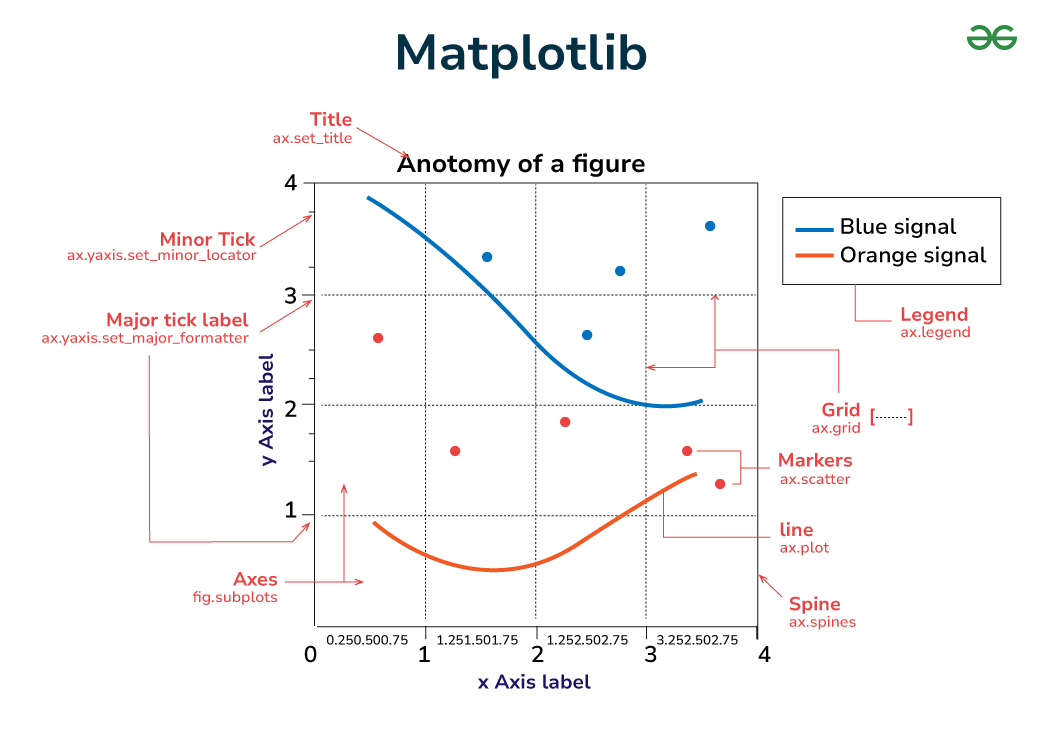
\includegraphics[width=0.8\textwidth]{Matplotlib.png}
\end{frame}

\section{Basic Components or Parts of Matplotlib Figure}

\begin{frame}
    \begin{itemize}
        \item \texttt{\color{red}Figures in Matplotlib:} The Figure object is the top-level container for all elements of the plot. It serves as the canvas on which the plot is drawn. You can think of it as the blank sheet of paper on which you’ll create your visualization.
        \item \texttt{\color{red}Axes in Matplotlib:} Axes are the rectangular areas within the figure where data is plotted. Each figure can contain one or more axes, arranged in rows and columns if necessary. Axes provide the coordinate system and are where most of the plotting occurs.
        \item \texttt{\color{red}Axis in Matplotlib:} Axis objects represent the x-axis and y-axis of the plot. They define the data limits, tick locations, tick labels, and axis labels. Each axis has a scale and a locator that determine how the tick marks are spaced.
    \end{itemize}
\end{frame}

\begin{frame}
    \begin{itemize}
        \item \texttt{\color{red}Adding lines to Figures:} Lines connect data points on a plot and are commonly used in line plots, scatter plots with connected points, and other types of plots. They represent the relationship or trend between data points and can be styled with different colors, widths, and styles to convey additional information.
        \item \texttt{\color{red}Matplotlib Title:} The title is a text element that provides a descriptive title for the plot. It typically appears at the top of the figure and provides context or information about the data being visualized.
        \item \texttt{\color{red}Marker in Matplotlib:} Markers are symbols used to denote individual data points on a plot. They can be shapes such as circles, squares, triangles, or custom symbols. Markers are often used in scatter plots to visually distinguish between different data points.
    \end{itemize}
\end{frame}

\begin{frame}
    \begin{itemize}
        \item \texttt{\color{red}Axis Labels in Matplotlib:} Labels are text elements that provide descriptions for the x-axis and y-axis. They help identify the data being plotted and provide units or other relevant information.
        \item \texttt{\color{red}Ticks:} Tick labels are text elements that provide labels for the tick marks. They usually display the data values corresponding to each tick mark and can be customized to show specific formatting or units.
        \item \texttt{\color{red}Matplotlib Legend:} Legends provide a key to the symbols or colors used in the plot to represent different data series or categories. They help users interpret the plot and understand the meaning of each element.
    \end{itemize}
\end{frame}

\begin{frame}
    \begin{itemize}
        \item \texttt{\color{red}Matplotlib Grid Lines:} Grid lines are horizontal and vertical lines that extend across the plot, corresponding to specific data intervals or divisions. They provide a visual guide to the data and help users identify patterns or trends.
        \item \texttt{\color{red}Spines of Matplotlib Figures:} 
        Spines are the lines that form the borders of the plot area. They separate the plot from the surrounding whitespace and can be customized to change the appearance of the plot borders.
    \end{itemize}
\end{frame}

\section{Different Types of Plots in Matplotlib}
\begin{frame}
    \begin{itemize}
       \item Matplotlib offers a wide range of plot types to suit various data visualization needs. Here are some of the most commonly used types of plots in Matplotlib:
       \item \texttt{\color{red}Line Graph, Stem Plot, Bar chart, \newline Histograms, Scatter Plot, Stack Plot \newline
       Box Plot, Pie Chart, Error Plot, Violin Plot, 3D Plots }
    \end{itemize}
\end{frame}


\begin{frame}
    \begin{center}
        {\Huge\ \color{red} Check notebook for more information and codes}
    \end{center}
\end{frame}
\begin{frame}
    \begin{center}
        {\Huge\ End of Visualization}
    \end{center}
\end{frame}

\end{document}

